\documentclass[onecolumn,10pt]{IEEEtran}
\let\labelindent\relax
\usepackage{enumitem}
\usepackage{etex}
\newcommand\hmmax{0}
\newcommand\bmmax{0}
\usepackage{amssymb,amsfonts,amsmath,amsthm}
\usepackage{graphicx}
\usepackage[usenames,x11names, dvipsnames, svgnames]{xcolor}
\usepackage{amsmath,amssymb}
\usepackage{dsfont}
\usepackage{amsfonts}
\usepackage{mathrsfs}
\usepackage{texshade}
\usepackage{hyperref}
\hypersetup{
  colorlinks=true,
  linkcolor=black,
  citecolor=black,
  filecolor=black,
  urlcolor=DodgerBlue4,
  breaklinks=false,
  % linkbordercolor=red,% hyperlink borders will be red
  % pdfborderstyle={/S/U/W 1}% border style will be underline of width 1pt
}
\usepackage{array}
\usepackage{xr}
\usepackage{verbatim}
\usepackage{multirow}
\usepackage{longtable}
\usepackage{siunitx}
\usepackage{booktabs}
\usepackage{tabularx}
\usepackage{ragged2e}

\usepackage{bm}
% \usepackage[T1,euler-digits]{eulervm}
% \usepackage{times}
% \usepackage{pxfonts}
\usepackage{tikz}
\usepackage{pgfplots}
\usetikzlibrary{shapes,calc,shadows,fadings,arrows,decorations.pathreplacing,automata,positioning}
\usetikzlibrary{external}
\usetikzlibrary{decorations.text}
\usepgfplotslibrary{colorbrewer} 
\usepgfplotslibrary{statistics}
\usetikzlibrary{shapes,calc,shadows,fadings,arrows,decorations.pathreplacing,automata,positioning}
\usetikzlibrary{shadows.blur}
\usetikzlibrary{fit}
\usepackage{comment}
\usepackage[size=normal]{subcaption}

\tikzexternalize[prefix=./Figures/External/]% activate externalization!
\tikzexternaldisable
% \addtolength{\voffset}{.1in}  
\usepackage{geometry}
\geometry{a4paper, left=.65in,right=.65in,top=.8in,bottom=0.7in}

\usepackage{pdflscape}

\addtolength{\textwidth}{-.1in}    
\addtolength{\hoffset}{.05in}    
\addtolength{\textheight}{.1in}    
\addtolength{\footskip}{0in}    
\usepackage{rotating}
\definecolor{nodecol}{RGB}{240,240,220}
\definecolor{nodeedge}{RGB}{240,240,225}
\definecolor{edgecol}{RGB}{130,130,130}
\tikzset{%
  fshadow/.style={      preaction={
      fill=black,opacity=.3,
      path fading=circle with fuzzy edge 20 percent,
      transform canvas={xshift=1mm,yshift=-1mm}
    }} 
}
\usetikzlibrary{pgfplots.dateplot}
\usetikzlibrary{patterns}
\usetikzlibrary{decorations.markings}
\usepackage{fancyhdr}
\usepackage{mathtools}
\usepackage{datetime}
\usepackage{comment}
%% ## Equation Space Control---------------------------
\def\EQSP{3pt}
\newcommand{\mltlne}[2][\EQSP]{\begingroup\setlength\abovedisplayskip{#1}\setlength\belowdisplayskip{#1}\begin{equation}\begin{multlined} #2 \end{multlined}\end{equation}\endgroup\noindent}
\newcommand{\cgather}[2][\EQSP]{\begingroup\setlength\abovedisplayskip{#1}\setlength\belowdisplayskip{#1}\begin{gather} #2 \end{gather}\endgroup\noindent}
\newcommand{\cgathers}[2][\EQSP]{\begingroup\setlength\abovedisplayskip{#1}\setlength\belowdisplayskip{#1}\begin{gather*} #2 \end{gather*}\endgroup\noindent}
\newcommand{\calign}[2][\EQSP]{\begingroup\setlength\abovedisplayskip{#1}\setlength\belowdisplayskip{#1}\begin{align} #2 \end{align}\endgroup\noindent}
\newcommand{\caligns}[2][\EQSP]{\begingroup\setlength\abovedisplayskip{#1}\setlength\belowdisplayskip{#1}\begin{align*} #2 \end{align*}\endgroup\noindent}
\newcommand{\mnp}[2]{\begin{minipage}{#1}#2\end{minipage}} 
%% COLOR DEFS------------------------------------------
\newtheorem{thm}{Theorem}
\newtheorem{cor}{Corollary}
\newtheorem{lem}{Lemma}
\newtheorem{prop}{Proposition}
\newtheorem{defn}{Definition}
\newtheorem{exmpl}{Example}
\newtheorem{rem}{Remark}
\newtheorem{notn}{Notation}
%% ------------PROOF INCLUSION -----------------
\def\NOPROOF{Proof omitted.}
\newif\ifproof
\prooffalse % or \draftfalse
\newcommand{\Proof}[1]{
  \ifproof
  \begin{IEEEproof}
    #1\end{IEEEproof}
  \else
  \NOPROOF
  \fi
}
%% ------------ -----------------
\newcommand{\DETAILS}[1]{#1}
%% ------------ -----------------
% color commands------------------------
\newcommand{\etal}{\textit{et} \mspace{3mu} \textit{al.}}
% \renewcommand{\algorithmiccomment}[1]{$/** $ #1 $ **/$}
\newcommand{\vect}[1]{\textbf{\textit{#1}}}
\newcommand{\figfont}{\fontsize{8}{8}\selectfont\strut}
\newcommand{\hlt}{ \bf \sffamily \itshape\color[rgb]{.1,.2,.45}}
\newcommand{\pitilde}{\widetilde{\pi}}
\newcommand{\Pitilde}{\widetilde{\Pi}}
\newcommand{\bvec}{\vartheta}
\newcommand{\algo}{\textrm{\bf\texttt{GenESeSS}}\xspace}
\newcommand{\xalgo}{\textrm{\bf\texttt{xGenESeSS}}\xspace}
\newcommand{\FNTST}{\bf }
\newcommand{\FNTED}{\color{darkgray} \scriptsize $\phantom{.}$}
\renewcommand{\baselinestretch}{.95}
\newcommand{\sync}{\otimes}
\newcommand{\psync}{\hspace{3pt}\overrightarrow{\hspace{-3pt}\sync}}
% \newcommand{\psync}{\raisebox{-4pt}{\begin{tikzpicture}\node[anchor=south] (A) {$\sync$};
%   \draw [->,>=stealth] ([yshift=-2pt, xshift=2pt]A.north west) -- ([yshift=-2pt]A.north east); %\end{tikzpicture}}}
\newcommand{\base}[1]{\llbracket #1 \rrbracket}
\newcommand{\nst}{\textrm{\sffamily\textsc{Numstates}}}
\newcommand{\HA}{\boldsymbol{\mathds{H}}}
\newcommand{\eqp}{ \vartheta }
\newcommand{\entropy}[1]{\boldsymbol{h}\left ( #1 \right )}
\newcommand{\norm}[1]{\left\lVert #1 \right\rVert}%
\newcommand{\abs}[1]{\left\lvert #1 \right\rvert}%
\newcommand{\absB}[1]{\big\lvert #1 \big\rvert}%
% #############################################################
% #############################################################
% PREAMBLE ####################################################
% #############################################################
% #############################################################
% \usepackage{pnastwoF}      
\DeclareMathOperator*{\argmax}{argmax}
\DeclareMathOperator*{\argmin}{arg\,min}
\DeclareMathOperator*{\expect}{\mathbf{E}}
\DeclareMathOperator*{\var}{\mathbf{Var}}

\newcommand{\ND}{ \mathcal{N}  }
\usepackage[linesnumbered,ruled,vlined,noend]{algorithm2e}
\newcommand{\captionN}[1]{\caption{\color{darkgray} \sffamily \fontsize{9}{10}\selectfont #1  }}
\newcommand{\btl}{\ \textbf{\small\sffamily bits/letter}}
\usepackage{txfonts}
% \usepackage{ccfonts}
%%% save defaults
\renewcommand{\rmdefault}{phv} % Arial
\renewcommand{\sfdefault}{phv} % Arial
\edef\keptrmdefault{\rmdefault}
\edef\keptsfdefault{\sfdefault}
\edef\keptttdefault{\ttdefault}

% \usepackage{kerkis}
\usepackage[OT1]{fontenc}
\usepackage{concmath}
% \usepackage[T1]{eulervm} 
% \usepackage[OT1]{fontenc}
%%% restore defaults
\edef\rmdefault{\keptrmdefault}
\edef\sfdefault{\keptsfdefault}
\edef\ttdefault{\keptttdefault}
\tikzexternalenable
% ##########################################################
\tikzfading[name=fade out,
inner color=transparent!0,
outer color=transparent!100]
% ###################################
\newcommand{\xtitaut}[2]{
  \noindent\mnp{\textwidth}{
    \mnp{\textwidth}{\raggedright\Huge \bf \sffamily #1}

    \vskip 1em

    {\bf \sffamily #2}
  }
  \vskip 2em
}
% ###################################
% ###################################
\tikzset{wiggle/.style={decorate, decoration={random steps, amplitude=10pt}}}
\usetikzlibrary{decorations.pathmorphing}
\pgfdeclaredecoration{Snake}{initial}
{
  \state{initial}[switch if less than=+.625\pgfdecorationsegmentlength to final,
  width=+.3125\pgfdecorationsegmentlength,
  next state=down]{
    \pgfpathmoveto{\pgfqpoint{0pt}{\pgfdecorationsegmentamplitude}}
  }
  \state{down}[switch if less than=+.8125\pgfdecorationsegmentlength to end down,
  width=+.5\pgfdecorationsegmentlength,
  next state=up]{
    \pgfpathcosine{\pgfqpoint{.25\pgfdecorationsegmentlength}{-1\pgfdecorationsegmentamplitude}}
    \pgfpathsine{\pgfqpoint{.25\pgfdecorationsegmentlength}{-1\pgfdecorationsegmentamplitude}}
  }
  \state{up}[switch if less than=+.8125\pgfdecorationsegmentlength to end up,
  width=+.5\pgfdecorationsegmentlength,
  next state=down]{
    \pgfpathcosine{\pgfqpoint{.25\pgfdecorationsegmentlength}{\pgfdecorationsegmentamplitude}}
    \pgfpathsine{\pgfqpoint{.25\pgfdecorationsegmentlength}{\pgfdecorationsegmentamplitude}}
  }
  \state{end down}[width=+.3125\pgfdecorationsegmentlength,
  next state=final]{
    \pgfpathcosine{\pgfqpoint{.15625\pgfdecorationsegmentlength}{-.5\pgfdecorationsegmentamplitude}}
    \pgfpathsine{\pgfqpoint{.15625\pgfdecorationsegmentlength}{-.5\pgfdecorationsegmentamplitude}}
  }
  \state{end up}[width=+.3125\pgfdecorationsegmentlength,
  next state=final]{
    \pgfpathcosine{\pgfqpoint{.15625\pgfdecorationsegmentlength}{.5\pgfdecorationsegmentamplitude}}
    \pgfpathsine{\pgfqpoint{.15625\pgfdecorationsegmentlength}{.5\pgfdecorationsegmentamplitude}}
  }
  \state{final}{\pgfpathlineto{\pgfpointdecoratedpathlast}}
}
% ###################################
% ###################################
\newcolumntype{L}[1]{>{\rule{0pt}{2ex}\raggedright\let\newline\\\arraybackslash\hspace{0pt}}m{#1}}
\newcolumntype{C}[1]{>{\rule{0pt}{2ex}\centering\let\newline\\\arraybackslash\hspace{0pt}}m{#1}}
\newcolumntype{R}[1]{>{\rule{0pt}{2ex}\raggedleft\let\newline\\\arraybackslash\hspace{0pt}}m{#1}}



% ################################################
% ################################################
% ################################################
% ################################################
% ####################################
\newcommand{\set}[1]{\left\{ #1 \right\}}
\newcommand{\paren}[1]{\left( #1 \right)}
\newcommand{\bracket}[1]{\left[ #1 \right]}
% \newcommand{\norm}[1]{\left\Vert #1 \right\Vert}
\newcommand{\nrm}[1]{\left\llbracket{#1}\right\rrbracket}
\newcommand{\parenBar}[2]{\paren{#1\,{\left\Vert\,#2\right.}}}
\newcommand{\parenBarl}[2]{\paren{\left.#1\,\right\Vert\,#2}}
\newcommand{\ie}{$i.e.$\xspace}
\newcommand{\addcitation}{\textcolor{black!50!red}{\textbf{ADD CITATION}}}
\newcommand{\subtochange}[1]{{\color{black!50!green}{#1}}}
\newcommand{\tobecompleted}{{\color{black!50!red}TO BE COMPLETED.}}


\newcommand{\pIn}{\mathscr{P}_{\textrm{in}}}
\newcommand{\pOut}{\mathscr{P}_{\textrm{out}}}
\newcommand{\aIn}[1][\Sigma]{#1_{\textrm{in}}}
\newcommand{\aOut}[1][\Sigma]{#1_{\textrm{out}}}
\newcommand{\xin}[1]{#1_{\textrm{in}}}
\newcommand{\xout}[1]{#1_{\textrm{out}}}

\newcommand{\R}{\mathbb{R}} % Set of real numbers
\newcommand{\F}[1][]{\mathcal{F}_{#1}}
\newcommand{\SR}{\mathcal{S}} % Semiring of sets
\newcommand{\RR}{\mathcal{R}} % Ring of sets
\newcommand{\N}{\mathbb{N}} % Set of natural numbers (0 included)


\newcommand{\Pp}[1][n]{\mathscr{P}^+_{#1}}
\renewcommand{\entropy}[1]{\boldsymbol{h}\left ( #1 \right )}

\def\TPR{\textrm{TPR}\xspace}
\def\TNR{\textrm{TNR}\xspace}
\def\FPR{\textrm{FPR}\xspace}
\def\PPV{\textrm{PPV}\xspace}

\usetikzlibrary{arrows.meta}
\usetikzlibrary{decorations.pathreplacing,shapes.misc}
\usepgfplotslibrary{fillbetween}
%usepackage{tikz-network}
\usetikzlibrary{shapes.geometric}
\usetikzlibrary{math}
\usepgfplotslibrary{colorbrewer} 

\usepackage{textcomp}
\usepackage{colortbl}
\usepackage{array}
\usepackage{courier} 
\usepackage{wrapfig}
\usepackage{pifont}
\usetikzlibrary{chains,backgrounds}
\usetikzlibrary{intersections}
\usetikzlibrary{pgfplots.groupplots}
\usepgfplotslibrary{fillbetween} 
\usetikzlibrary{arrows.meta}
\usepackage{pgfplotstable}
\usepackage[super,compress,sort,comma]{natbib}

\usepackage{setspace}
\usetikzlibrary{math}
\usetikzlibrary{matrix}
\usepackage{xstring}
\usepackage{xspace}
\usepackage{flushend}

\makeatletter
\renewcommand\section{\@startsection {section}{1}{\z@}%
  {-2ex \@plus -1ex \@minus -.2ex}%
  {1ex \@plus.1ex}%
  {\Large\bfseries\scshape}}
\renewcommand\subsection{\@startsection {subsection}{1}{\z@}%
  {-2ex \@plus -.25ex \@minus -.2ex}%
  {0.1ex \@plus.0ex}%
  {\fontsize{11}{10}\selectfont\bfseries\sffamily\color{black}}}
\renewcommand\subsubsection{\@startsection {subsubsection}{1}{\z@}%
  {0ex \@plus -.5ex \@minus -.2ex}%
  {0.0ex \@plus.5ex}%
  {\fontsize{9}{9}\selectfont\bfseries\itshape\sffamily\color{darkgray}}}
\renewcommand\paragraph{\@startsection {paragraph}{1}{\z@}%
  {-.2ex \@plus -.5ex \@minus -.2ex}%
  {0.0ex \@plus.5ex}%
  {\fontsize{9}{9}\selectfont\itshape\sffamily\color{darkgray}}}
       
%\renewcommand{\thesubsection}{\thesection.\arabic{subsection}}
\renewcommand{\thesubsectiondis}{\arabic{subsection}.}
\renewcommand{\thesectiondis}{\arabic{section}.}
\renewcommand{\thesection}{\arabic{section}}

\renewcommand{\thetable}{\arabic{table}}

\makeatother
\makeatletter
\pgfdeclareradialshading[tikz@ball]{ball}{\pgfqpoint{-10bp}{10bp}}{%
  color(0bp)=(tikz@ball!30!white);
  color(9bp)=(tikz@ball!75!white);
  color(18bp)=(tikz@ball!90!black);
  color(25bp)=(tikz@ball!70!black);
  color(50bp)=(black)}
\makeatother
%\newcommand{\tball}[1][CadetBlue4]{${\color{#1}\Large\boldsymbol{\blacksquare}}$}
\renewcommand{\baselinestretch}{1}
%\renewcommand{\captionN}[1]{\caption{\color{CadetBlue4!50!black} \sffamily \fontsize{9}{10}\selectfont #1  }}
\tikzexternaldisable 
\parskip=6pt
\parindent=0pt
%\newcommand{\Mark}[1]{\textsuperscript{#1}}
\pagestyle{fancy}

\newcounter{Dcounter}
\setcounter{Dcounter}{1}
\newcommand{\DQS}[1]{\marginpar{\tikzexternaldisable \tikz{\node[rounded corners=5pt,draw=none,thick,fill=black!10,font=\sffamily\fontsize{7}{8}\selectfont] {\mnp{.45in} {\color{Red3}\raggedright  \#\theDcounter.~#1}}; }}\stepcounter{Dcounter}\xspace}

\newcommand{\qn}[1][i]{\Phi_{#1}}
\newcommand{\D}[1][i]{\mathscr{D}\left ( {\Sigma_#1} \right ) }
\newcommand{\Dx}{\mathscr{D}}
\def\J{\mathds{J}}
\def\M{\omega}
\def\N{\mathds{N}}
\newcommand{\cp}[1][P]{\langle #1 \rangle}
\newcommand{\mem}[1]{\M_{#1}}


\makeatletter
\newcommand\transformxdimension[1]{
    \pgfmathparse{((#1/\pgfplots@x@veclength)+\pgfplots@data@scale@trafo@SHIFT@x)/10^\pgfplots@data@scale@trafo@EXPONENT@x}
}
\newcommand\transformydimension[1]{
    \pgfmathparse{((#1/\pgfplots@y@veclength)+\pgfplots@data@scale@trafo@SHIFT@y)/10^\pgfplots@data@scale@trafo@EXPONENT@y}
}
\makeatother

\parskip=6pt
\parindent=0pt


\pgfplotsset{
    discard if/.style 2 args={
        x filter/.code={
            \edef\tempa{\thisrow{#1}}
            \edef\tempb{#2}
            \ifx\tempa\tempb
                \def\pgfmathresult{inf}
            \fi
        }
    },
    discard if not/.style 2 args={
        x filter/.code={
            \edef\tempa{\thisrow{#1}}
            \edef\tempb{#2}
            \ifx\tempa\tempb
            \else
                \def\pgfmathresult{inf}
            \fi
        }
    }
  }

\def\commatononei#1,{#1}
\def\commatononej#1,#2,{#1#2}
\def\commatonone#1{\expandafter\commatononei#1}
\def\commatononeT#1{\expandafter\commatononej#1}
\newcommand{\Sum} [2] {#1 + #2 = \the\numexpr #1 + #2 \relax \\}

\newcounter{Ccounter}
\setcounter{Ccounter}{1}
\newcommand{\comm}[1]{{\color{gray} {\bf \sffamily Comment~\#\theCcounter.~}#1}\xspace}
\newcommand{\resp}[1]{{\color{Blue2} {\bf \sffamily Author Response~\#\theCcounter.~}#1}\stepcounter{Ccounter}\xspace}

\usepackage{float}
%\usetikzlibrary{decorations.pathreplacing,calligraphy}
\def\TITLE{[Ve]tting  [R]esponse [I]ntegrity from  \\cross-[T]alk  dependencies in [A]dversarial [S]urveys: \\ \itshape ``Who can catch a liar?''}

\title{\TITLE}

\def\x{\bm{\mathrm{x}}} 
\def\y{\bm{\mathrm{y}}}

\author{\sffamily  \fontsize{10}{12}\selectfont Robert Gibbons,       Ishanu Chattopadhyay$^{1,4,5,7\bigstar}$\\ 
\vspace{10pt}

\sffamily  \fontsize{10}{12}\selectfont
$^{1}$Department of Medicine, University of Chicago, Chicago, IL 60637, USA\\ 
$^{4}$Committee on Quantitative Methods in Social, Behavioral, and Health Sciences, University of Chicago, Chicago, IL 60637, USA\\
$^{5}$Committee on Genetics, Genomics \& Systems Biology, University of Chicago, Chicago, IL 60637, USA
\vskip 1em
$^\bigstar$To whom correspondence should be addressed: e-mail: \href{mailto:ishanu@uchicago.edu}{\texttt{ishanu@uchicago.edu}}.}
\title{\TITLE}


\def\TEXTCOL{gray}



\def\J{\mathds{J}}
\def\M{\omega}
%\newcommand{\mem}[1]{\M_{#1}}
\def\cognet{CogNet\xspace}
\def\qnet{Q-net\xspace}
\def\qdist{q-distance\xspace}
\def\qbiome{Qbiome\xspace}
\def\qsamp{q-sampling\xspace}

\def\x{\bm{\mathrm{x}}}
\def\y{\bm{\mathrm{y}}}
\def\erisk{$M_\delta$\xspace}
\def\RHO{A_\delta}
\def\bact{Bacteroidia\xspace}
\def\actn{Actinobacteria\xspace}
\def\gamm{Gammaproteobacteria\xspace}
\def\ubac{unclassified Bacteria\xspace}
\def\bacl{Bacilli\xspace}
\def\clsd{Clostridia\xspace}
\def\corb{Coriobacteriia\xspace}
\def\verru{Verrucomicrobia\xspace}

\renewcommand{\baselinestretch}{.97}
%\externaldocument[SI-]{SI}
%\externaldocument[main-]{main}
% \externaldocument[EXT-]{exfig}
\newif\iftikzX
\tikzXtrue
\tikzXfalse
\newif\ifFIGS  
\FIGSfalse  
\FIGStrue
\cfoot{\scriptsize\thepage}
\lfoot{}
\rfoot{} 
\def\EXTENDEDDATA{Extended Data\xspace}
\def\SUPPLEMENTARY{Supplementary\xspace}
\def\Methods{Online Methods}
\def\SPREFIX{S-}
\def\SPREFIX{}
\def\SUPPLEMENTARY{Extended Data\xspace}

\pgfplotsset{compat=1.16}


\def\vrts{\texttt{VeRITAS}\xspace}

\begin{document}
\maketitle
 

{\bf \sffamily \fontsize{10}{12}\selectfont \noindent   
  {\normalfont \itshape Abstract:} Animal influenza  viruses emerging into humans % are suspected to
  have triggered devastating  pandemics in the past~\cite{shao2017evolution,mills2004transmissibility,reid2003origin,landolt2007up}. Yet, our ability to evaluate the pandemic potential of individual strains that do not yet circulate in humans, remains limited. In this study we introduce the \qnet, to computationally learn how new variants emerge, shaped by evolutionary constraints using only observed genomic sequences  of key viral proteins. }
  
\vspace{10pt} 

\section*{Introduction}
Diagnosis of mental health disorders often rely heavily on self-reporting or structured interviews~\cite{ali2015multimodal}, which opens up the possibility of  intentional fabrication of  symptoms~\cite{Rogers1997,rogers2008clinical}, referred to as ``malingering'', or untruthgful answers arising from some underlying mental diseas or even socio-economic compulsion [REF]. In the specific context of diagnosing Post-Traumatic Stress Disorder (PTSD),  subjective stressors combined with  similarity in presentation across patients, the easily availability of  information on  how to fake PTSD, % and substantial incentives to malinger  for individuals involved in criminal or civil procedures or   disability claims,
is known to confound  accurate  assessments.  


Clinically, PTSD is an anxiety disorder that can develop after experiencing a traumatic event. In the United States,  substantial disability compensation may be  available for  those with mental disorders including PTSD, which while being an crucial resource for the truely afflicted, incentivizes malingering behavior~\cite{frueh2007us,taylor2007detection}.  Some might also fake PTSD to access medical treatment, commit insurance, personal injury and other frauds,  or in an attempt to evade criminal liability and penalties~\cite{guriel2003assessing,salloway1990opiate,resnick2008malingering,burkett1998stolen}. Thus, while on one hand, PTSD is a serious mental health condition  associated with comorbid substance use disorder, mood disorder, anxiety disorder,  personality disorder, increased morbidity,  and possibly with increased  mortality~\cite{goldstein2016epidemiology,schnurr2009posttraumatic}, false  diagnoses cause substantial financial drain~\cite{lopiccolo1999current} to the healthcare system, and  the VA~\cite{oboler2000disability}, diverts crucial resources from where they are needed~\cite{taylor2006clinician}, and interfere with study outcomes by introducing inaccuracies in clinical data~\cite{rosen2006dsm}. Accurate disambiguation of true and fake PTSD is therefore  of high importance, especially with sources suggesting that over 20\% of  personal injury cases, as well as  20\%  of the Veterans seeking combat compensation could be  fabricating their condition~\cite{marx2011ptsd,rogers1994explanatory,leeshaley1997mmpi2,frueh2007us}.

Briefly state the medical side of things, that people might be faking PTSD for other clinical reasons.

Multiple standardized tests~\cite{Wong2005,smith1997detection} and  validity assessment tools~\cite{ben2012interpreting} have been explored  for malingering detection with limited success. These tools typically aim to incorporate patterns observed in diagnostic populations that might disambiguate faked symptoms from real ones. However,  existing approaches  do not target specific disorders, require expert interpretation, are often subjective, and by design are  unlikely to be effective against a malingerer with psychiatric training (See Table~\ref{tbl:methods_summary}). Other  strategies that incorporate diverse physiological monitoring and linguistic analysis~\cite{ekman1991who,mihalcea2009lie,burgoon2008cognitive,zhou2004automating}  cannot be easily  adopted  in the present context of structured or semi-structured interviews.

Here we introduce an AI-driven approach to flag malingering participants in structured interviews, demonstrated in the context of PTSD diagnosis. We leverage the fact that
responses to  items  in a structured interview have emergent statistical dependencies  arising from the nature of the questions, and are modulated by the presence of the trait we are aiming to detect $e.g.$, PTSD pathology. These dependencies are too
complex to easily preempt and replicate on-the-fly, even with knowledge about how such patients tend to respond $i.e.$ with training in the mental health services. We find that an ``algorithmic lie detector'' that exploits this structure inferred from historical response databases, is  difficult to defeat, and offers a robust generalizable approach to verifying response validity. Algorithm \vrts can be tuned to target malingering in specific disorders, can be rapidly trained from historical data, can be administered easily, and require subtantially less subjective interpretation, and presents a generative AI's take on Ekman's paper ``Who Can Catch a Liar?''~\cite{Ekman1992}.



\begin{figure}
  \tikzexternalenable
  \tikzsetnextfilename{scheme}
    \centering
\tikzXtrue
 \iftikzX  
    \begin{tikzpicture}
    \node [] (A) at (0,0) {
      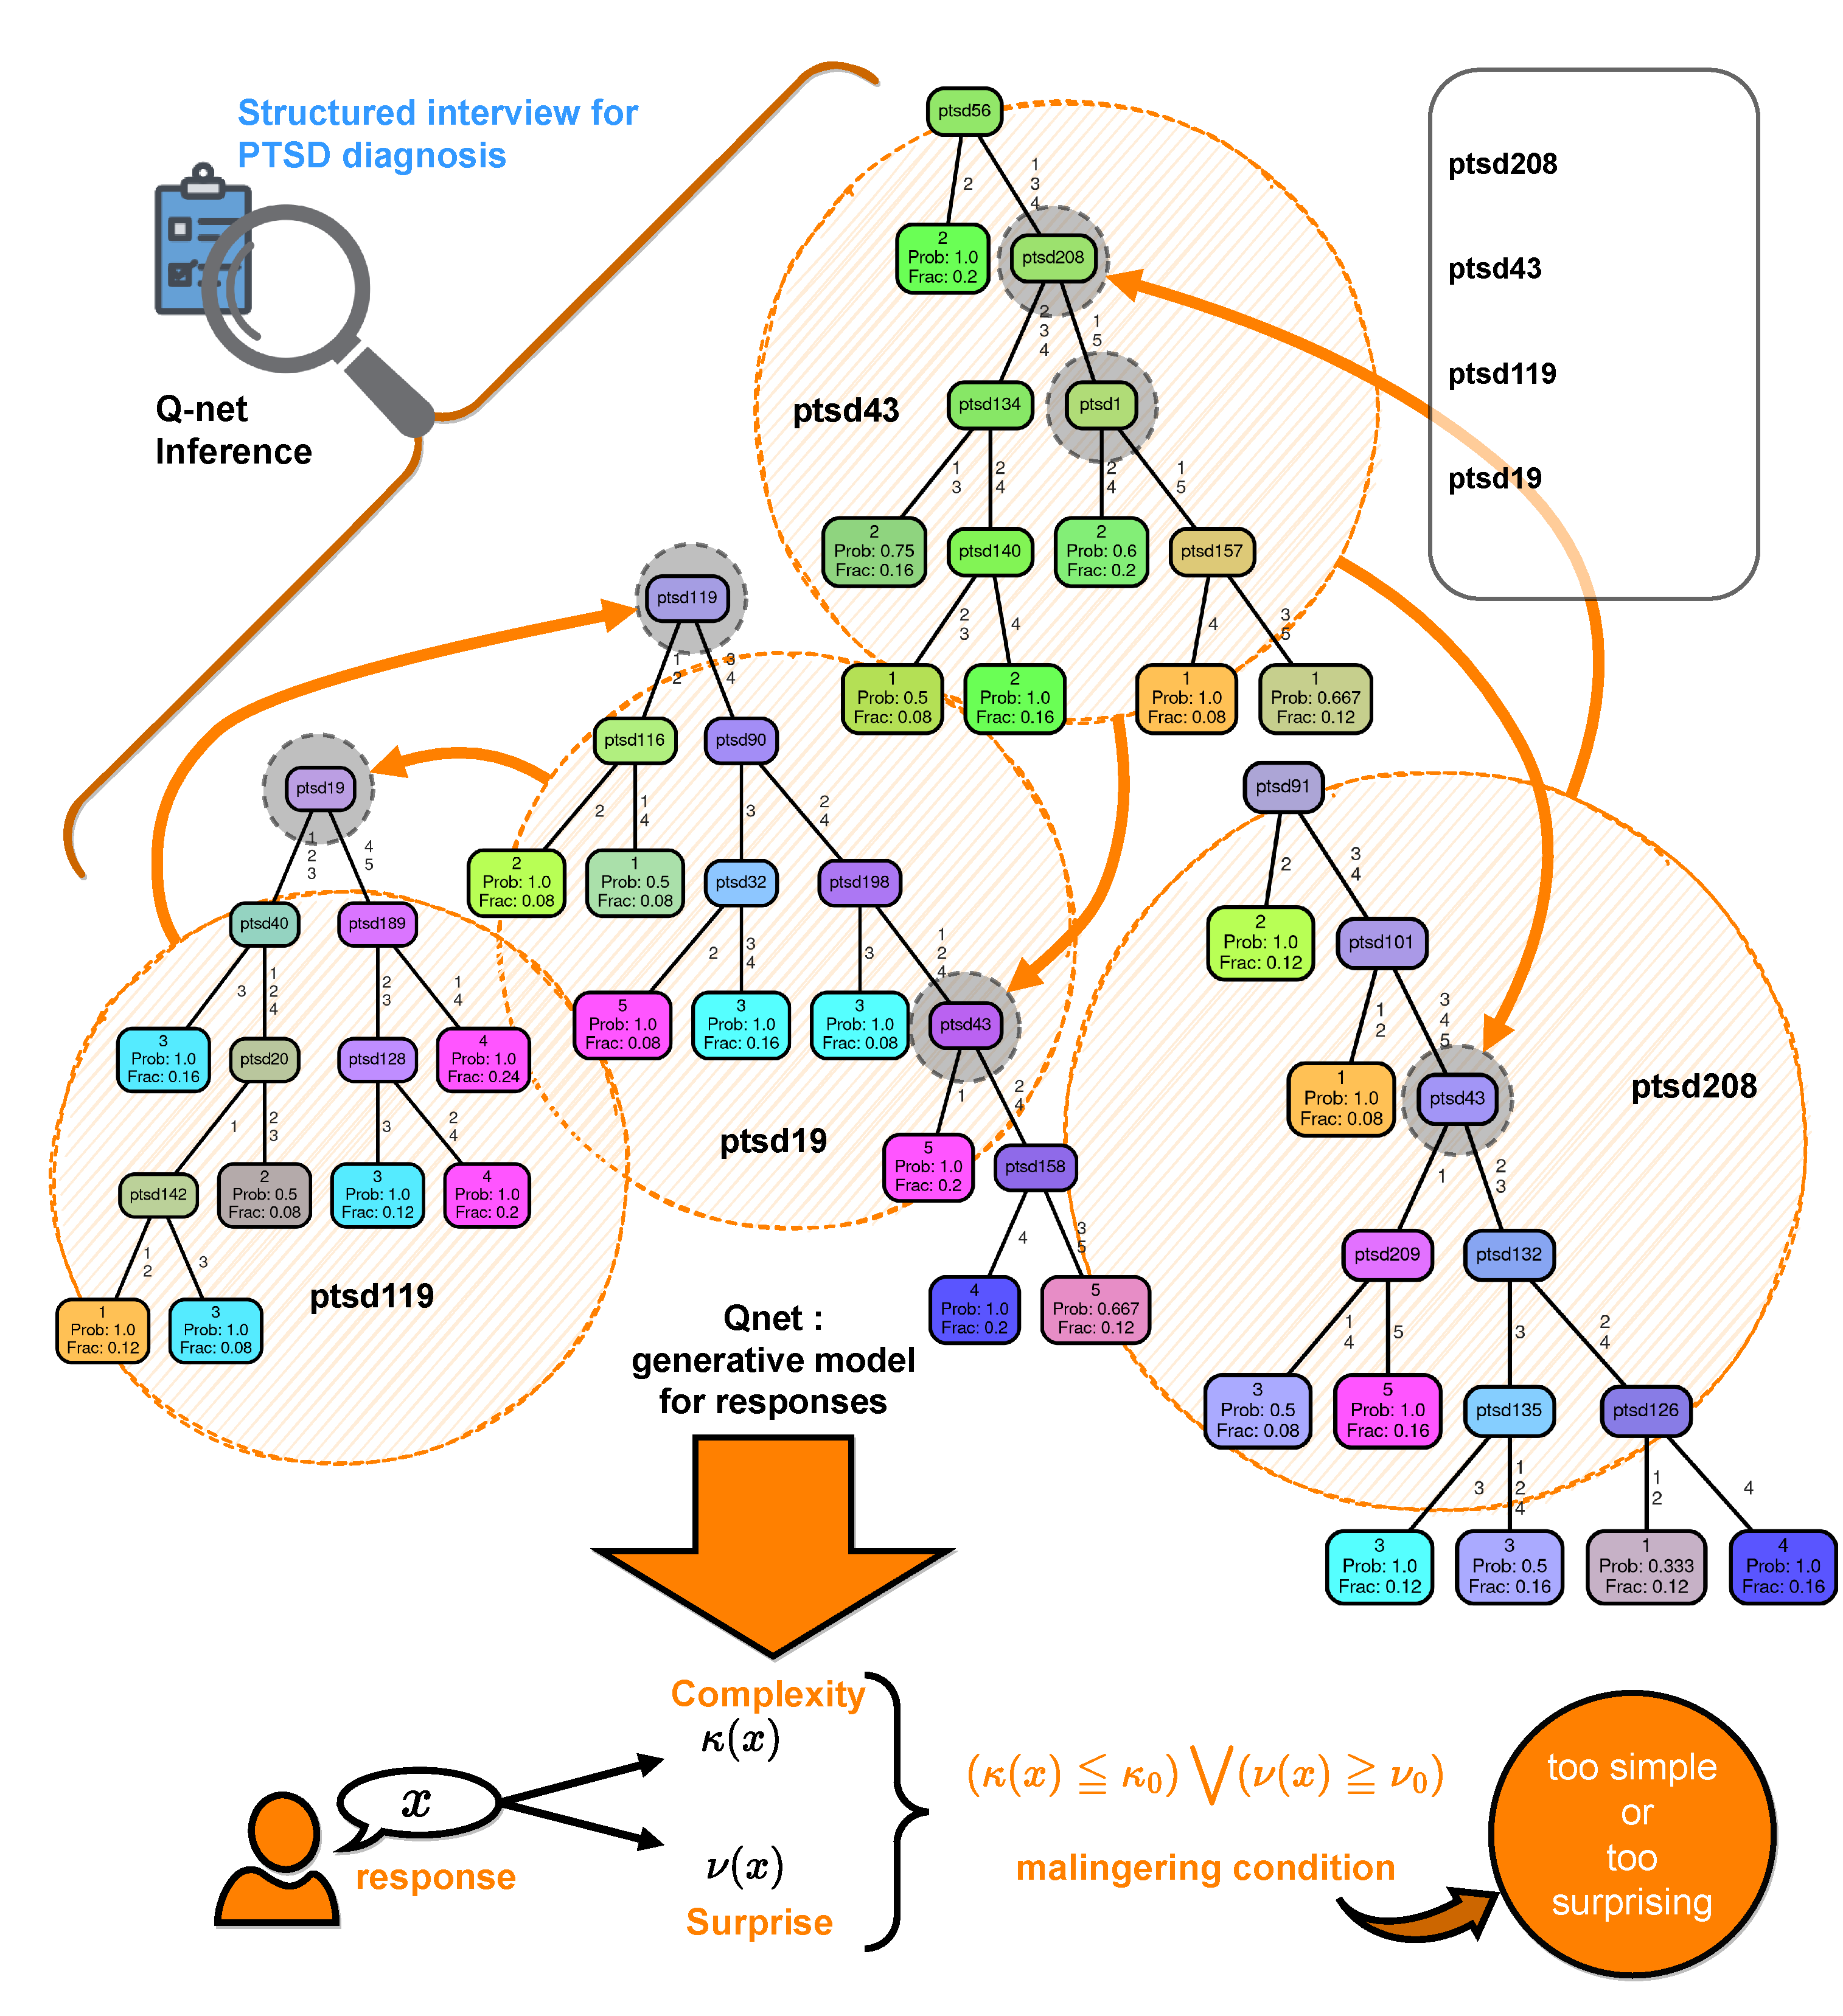
\includegraphics[width=\textwidth]{Figures/qnetptsd}};
    \node [] (B) at ([yshift=1.65in,xshift=-2.35in]A.south) {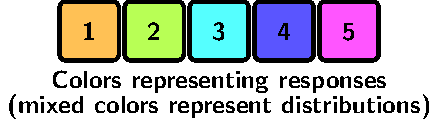
\includegraphics[width=2in]{Figures/test}};
    % \node [text=gray,font=\bf\sffamily\fontsize{8}{8}\selectfont] (C) at ([yshift=7.65in,xshift=-.2in]A.south) {\mnp{6.5in}{\begin{tabular}{C{.25in}L{1.6in}}
  ptsd19 & Feel emotionally numb due to a stressful event in the past?\\
  ptsd43 & Still enjoy doing many things that you used to enjoy? \\
  ptsd119& How often have you experienced memory problems due to a stressful event in the past? \\
\end{tabular}                         }};
                                                                    \end{tikzpicture}
                      
 \else
  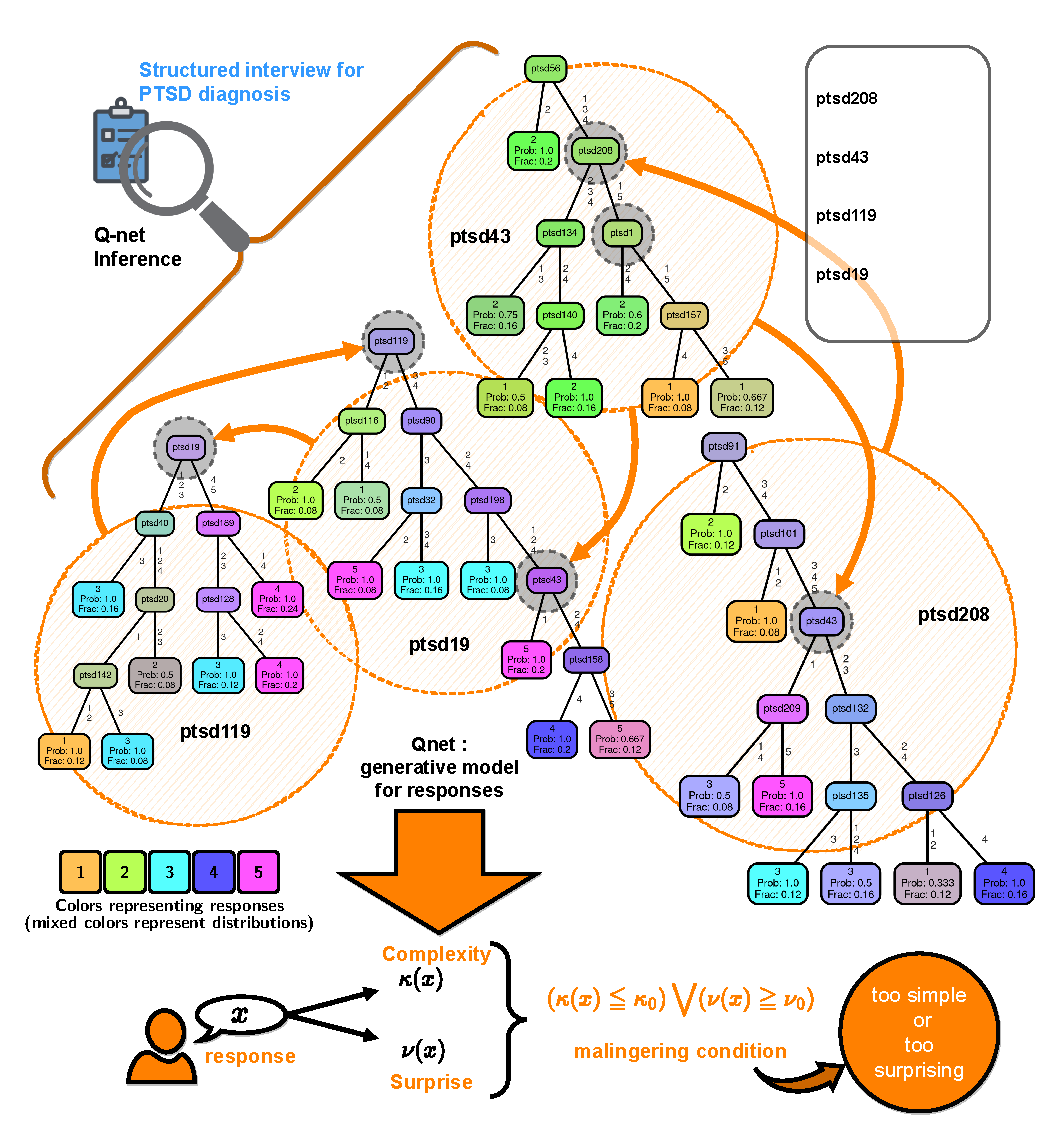
\includegraphics[width=\textwidth]{Figures/External/scheme}
  \fi
                                              \captionN{}\label{qnet}
                                                                  \end{figure}

\section*{Results} 

\subsection*{Participants and Data Sources}
The interview data used in training in this study  consists of  $n=304$ participants  recruited at a Veterans Health Administration facility for an earlier study~\cite{brenner2021development}. Veterans were eligible if they were between the ages of 18 and 89 years and able to provide written informed consent. Once eligibility was determined by the study team, participants completed a PTSD-symptom questionnaire from the CAT-PTSD item bank~\cite{gibbons2012development,brenner2021development} (comprising $211$ items) and provided responses on the PTSD Checklist for Diagnostic and Statistical Manual of Mental Disorders, Fifth Edition (DSM-5) (PCL-5). Participants in teh training dataset were interviewed using the Clinician-Administered Scale for PTSD for DSM-5 ($86$ were diagnosed, $218$ were deemed  PTSD-negative).

\subsection*{Key Insight}
Our key insight  is that malingered responses  have low likelihood of being generated while respecting the emergent cross-dependencies. The proposed framework enables verifying this condition efficiently without strong a priori assumptions of the nature and structure of these cross-dependencies. This condition can also be thought of as stipulating that malingered responses have high average ``surprise'', $i.e. $ deviate more on average from the model predictions of item responses. We learn a generative model for responses to structured diagnostic interviews that can discover $n$-way dependencies between the items. Finally, we aim to robustly flag malingering by checking if two specific  response attributes $\kappa, \nu$ related to likelihood and surprise violate preset thresholds.

\subsection*{\qnet Inference and Cross-talk Modeling}


\subsection*{Training and Validation}

\subsection*{Performance}

\subsection*{Comparison Against State of Art}



\section*{Discussion}
Malingering remains a persistent problem, especially in psychiatric and criminal justice settings, with prevalence estimates ranging from $8-64\%$\cite{mcdermott2013malingering,schmidt2020base,matto2019systematic}. Here we develop a novel system to address this gap for  the need for further development of reliable, rigorous, and principled methods for detecting deception remains highly significant~\cite{DePaulo2003}.

{\color{Red1} In this study, we introduce a novel algorithmic technique for identifying  deception in structured interviews. This approach first infers a detailed model of the response patterns of previous respondents, then uses a measure of consistency known as dissonance to identify if future respondents' answers are indicative of deception.}

Our model-based, data-driven approach is notably distinct from traditional methods of malingering detection, which are typically constructed for  specific contexts~\cite{walczyk2018review}. in the context of  psychiatric diagnosis detection of faked symptoms is often based on standardized tests; some commonly used ones are summarized in Table \ref{tbl:methods_summary}. Tests such as the Structures Interview of Reported Symptoms (SIRS)~\cite{Wong2005}, Structured Inventory of Malingered Symptomology (SIMS)~\cite{smith1997detection}, and the Minnesota Multiphasic Personality Inventory-2 and its associated validity scales~\cite{ben2012interpreting} draw extensively on research of both legitimate psychiatric patients and malingerers, and employ a combination of detection strategies focused on symptoms that are either unlikely to be presented by genuine patients, or that tend to be amplified in malingerers~\cite{rogers2008determinations}. For detection of cognitive malingering, physiological, arousal-based approaches such as the Control Question Technique\cite{vrij2001killed}, and cognitive load-inducing approaches such as requiring subjects to perform a concurrent task ($e.g.$ maintaining eye contact) and the Autobiographical Implicit Association Test (aIAT) have been suggested.

Accuracy rates for these research-driven state of the art detection techniques are typically in the range of $85$-$95$\% depending on the specific problem context\cite{sartori2008accurately,gregg2007vying,monaro2017detection} (similarly high sensitivities have also been reported \cite{smith1997detection}). However, among the limitations to these methods is the requirement of substantial domain research and/or subject matter expertise to develop. Thus while these methods perform well in the specific context for which they were developed, it may be challenging and/or expensive to broadly extend to detection in other contexts. In the case of cognitive malingering methods, vulnerabilities to clinician/adminstrator bias, high rates of false positives and false negatives, and vulnerability to coaching have been noted as possible limitations. 

In contrast with these methods, our results demonstrate that it is possible to achieve similar (or perhaps improved) performance in detecting malingering by identifying structural differences in an individual's responses compared to a set of baseline responses. The basic insight underpinning our results is that consistent, genuine responses to interview questions are typically not independent. In general, there are dependence patterns between interview questions, which are often nontrivial and difficult or impossible to identify a priori. Given the entirety of responses an individual has provided in an ongoing interview, the response probabilities for a consistent response to the next question are governed by these dependence patterns. As these probabilistic constraints exist between all questions in the interview, a complex interaction network is induced over the high-dimensional response space. To infer the structure of this network, we use a novel architecture - the \qnet, a nonparametric generative model of the response network which reflects the $n$-way inter-question relations found amongst previous interview respondents.

From the model's approximation of the probabilistic dependencies present in the response network, we derive the dissonance as an intuitive, individually computable measure of response consistency. For all data sets in this study, mean dissonance values for random malingering and expert malingering are significantly higher than for actual responses, empirically demonstrating its utility for identifying such responses. As should be expected, we also found that the expert malingering responses were on average less dissonant than random malingering, showing that domain knowledge does allow individuals to respond in a more convincing manner. However, their failure to adequately account for detailed inter-question dependencies tends to make their responses significantly different from actual responses in a measurable, quantitative sense. 

The classification results obtained further demonstrate the ability of this framework to identify subtle deviations in the response patterns of actual and malingering respondents. Due to the lower dissonance generated by expert malingerers, we found it more difficult to identify such responses; however, in practice it appears unlikely that even the most knowledgeable domain experts would have the requisite quantitative knowledge of response distributions of the target phenotype to be able to respond in the manner of our idealized expert malingerers. Thus in real-world usage where true malingerers are likely a mixture of these two idealizations, we would expect performance to be bounded above and below by the empirical performance obtained for the random and expert scenarios.

In general, data-driven methods for detection of malingering are not as ubiquitous as in other domains; however, the increasing availability of modern sensory data collection has allowed for implementation of machine learning algorithms and computer vision techniques~\cite{Chan2018, Wang2020, Lee2019} for detecting deception based on patterns in language, facial expressions, body movements, and eye movements~\cite{Yu2018, Ducharme2017}. These methods have been shown to outperform traditional lie detection methods in some cases, obtaining accuracy rates of over 90\% for lie detection from patterns in facial expressions and body movements~\cite{Ekman1992,Yu2018} and 60-80\% using analysis of gaze direction and pupil dilation~\cite{Ducharme2017}%\cite{Granziero2019}.
. However, in many instances it is not feasible to collect detailed sensory data, possibly limiting the general applicability of these kinds of methods. By exclusively utilizing response data, our dissonance-based approach is not subject to such limitations.

%The basis of our algorithmic approach is a detailed model of the complex probabilistic dependencies present between an individual's responses to an interview question. Given that a response to a question is truthful, probabilities of subsequent responses to other related questions are changed. A priori, such dependencies are present amongst all possible questions in a given interview, which yields a combinatorial explosion of interactions to consider. For the PTSD data set, we have $211$ questions, which means that each individual's responses may be identified with a point in a $211$-dimensional space where the response to each question in principle depends on the other $210$ questions.

In contexts such as these, where malingerers seek to obtain a target diagnosis, training data from past respondents often includes a clinical phenotype for each respondent. However, this is not always available (as was observed for the CCHHS data set). Nonetheless, in the absence of the underlying diagnostic phenotypes, our approach still appears to perform well under a scenario in which expert malingerers are also unsure of ground-truth diagnoses. 

In other types of structured interviews, such as internet surveys and opinion polls, built-in data validity checks are frequently used to attempt to proactively identify disingenuous respondents. Among such checks, unusually fast response times have been observed to be indicative of poor data quality\cite{malhotra2008completion,callegaro2009response}, demonstrating a lack of attention by interview respondents\cite{greszki2015exploring}. Our finding of a negative correlation between dissonance and response time adds some support to this notion. However, it has been noted that duration-based validity checks may be vulnerable to a high false negative rate\cite{kennedy2020assessing}, suggesting a need for most robust measures of assessing validity. 

\section*{Methods}

\section{Definitions \& Notation}

\begin{defn}[Survey]
A survey for the purpose of this work is a structured interview, consisting of a finite number of questions (items) posed to a set of participants, with these items drawn from a finite item bank, and  whose responses must be one froma pre-specified set fo choices, $e.g.$, the Likert scale, with missing values for the responses allowed. 
\end{defn}


\begin{defn}[Response vector]
A response vector is the set of responses to a survey from a single participant, typically assuming that not all items are posed, and allows for the possibility that some responses are missing.
\end{defn}


A \qnet, as described here, is a model of the response dependency  structure for questions (items) posed to participants in a survey.  The \qnet explicitly estimates individual conditional distributions of each item response, which collectively serve as a model of the full joint distribution of the responses. 

\begin{defn}[\qnet]
\label{def:qnet}
Let $X \sim P$ be an $n$-dimensional discrete random vector supported on a finite set $\Sigma$ and following distribution $P$, i.e. \[X = (X_1, \ldots, X_n) \sim P, \hspace{0.25in} \operatorname{supp}(X) =  \Sigma = \displaystyle\prod_{i=1}^n \Sigma_i \hspace{.1in} \text{with } |\Sigma| < \infty.\] For $i = 1, \ldots, n$, let $P_i := P(X_i\,|\,X_j=x_j \text{ for } j \neq i)$ denote the conditional distribution of $X_i$ given the values of the other components of $X$.  Finally, for each $i = 1, \ldots, n$, let $\Phi^P_i$ denote an estimate of the distribution $P_i$.  Then the set $\Phi^P := \{\Phi^P_i\}_{i=1}^n$ is called a \emph{Quasinet (\qnet)}. Identifying the true distribution $P$ as the one describing the joint statistics of the responses from a survey with $n$ items, we also refer to  $\Phi^P$ as the \qnet for the survey $P$.
\end{defn}

When $P$ is clear from context, we may omit the superscript and simply write $\Phi = \{\Phi_i\}$ to denote the \qnet. The motivation for Definition \ref{def:qnet} is that the collection of all estimators $\Phi = \{ \Phi_i \}$ contained in a \qnet represents the set of all inferred dependencies from the observed ecosystem.  While the definition allows for arbitrary method of algorithm to construct the estimators $\Phi_i$, the utility of a \qnet clearly depends primarily on the properties of the $\Phi_i$.  In this study, we aim to minimize the set of a priori assumptions on the overall model structure to allow the complex dependencies present in $P$ to emerge. To that end, throughout this work all {\qnet}s are computed using conditional inference trees~\cite{sarda2017conditional} (a variant of classification and regression trees) to compute each $\Phi_i$. In general each \qnet component $\Phi_i$ is computed independently from the other $\Phi_j$, which allows a network structure to emerge amongst these estimators.

An important quantity for an inferred \qnet is the persistence function $\mem{\x}$.

%
\begin{defn}[Persistence Function]\label{def:mem}
Given a survey $P$ inducing the \qnet $\Phi^P$ and a response  vector $\x = (x_1, \ldots, x_n)$, the persistence $\mem{\x}$ of  $\x$ in the population modeled  by the \qnet:
\cgather{
\mem{\x}^P := \operatorname{Pr}(\x \in P) = \prod_{i=1}^n  \Phi^P_i(X_i = x_i\,|\,X_j = x_j, j \neq i) %
}%
\end{defn}
The persistence function $\mem{\x}^P$, as the name suggests,  is the probability that $\x$ persists, $i.e.$,  $Pr(\x \rightarrow \x)$ for the population modeled by the \qnet $P$, with $1-\mem{\x}^P$ being the probability that $\x$ is altered by a  random perturbation.

We will show  that if for two inferred \qnet models $P,Q$, we have $\mem{\x}^P \geqq \mem{\x}^Q$, then it is more likely that model $P$ generated $\x$. This is an important result that justifies the definition of the
score parameter in Defn.~\ref{defvrts}.

% \begin{wrapfigure}[16]{r}{1.7in}
%   \centering

%   \vspace{-17pt}
  
%   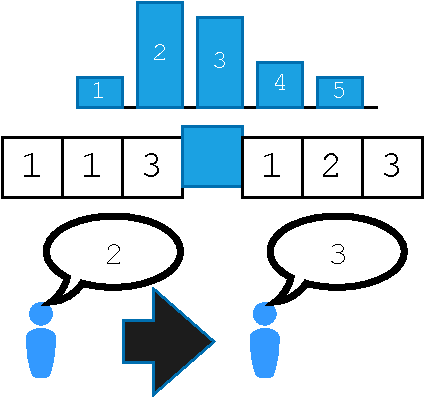
\includegraphics[width=1.65in]{Figures/responsecartoon.pdf}
%   \captionN{Why response vectors might change spontaneously: if  response to an item is a   sample from a  distribution over the possible responses, two responses with similar probabilities  can switch easily, thus making a spontaneous perturbation possible. }\label{figcartoon}
% \end{wrapfigure}
The \qnet allows us to rigorously compute  bounds on  the probability of a spontaneous change from one response vector to another, induced by spontaneous chance variations (Fig~\ref{figcartoon}). Not all perturbations in a vector are either likely or contextually meaningful. With an exponentially exploding number of possibilities in which a vector over a large set of items can vary, it is computationally intractable to directly model all possible dependecies; nevertheless, we can constrain the possibilities using the patterns we uncover via the \qnet construction.  A key piece of this approach is to design  an intrinsic distance between response vectors, which is reflective of this underlying  dependency structure.  

\begin{defn}[\qdist]
\label{defqdistance} 
Let $\Phi^P = \{\Phi_i^P\}_{i=1}^n$ and $\Phi^Q = \{\Phi_i^Q\}_{i=1}^n$ denote {\qnet}s on populations $P$ and $Q$, and suppose $\x=(x_1, \ldots, x_n)$ and $\y =(y_1, \ldots, y_n)$ are samples of $X \sim P$ and $Y \sim Q$ respectively. Then the \qdist $\theta_{P,Q}(\x,\y)$ between $\x$ and $\y$ is\[\theta_{P,Q}(\x,\y) := \frac{1}{n}\sum_{i=1}^n \left[ \mathbb{J}^{\frac{1}{2}} \left(\Phi_i^P(X_i |X_j = x_j, j \neq i) \,\|\, \Phi_i^Q(Y_i|Y_j = y_j, j \neq i\right ) \right]\]%
where $\mathbb{J}$ denotes the Jensen-Shannon divergence~\cite{cover}.
\end{defn}

For brevity, we may write simply $\theta$ (dropping the suffixes) if the populations are clear from context.  Since the Jensen-Shannon distance $\mathbb{J}$ is a legitimate metric~\cite{fuglede2004jensen} on the set of probability distributions (unlike KL-divergence), $\theta$ inherits nonnegativity, symmetry, and respects the triangle inequality; it follows that \qdist is a (pseudo)-metric on $\Sigma$. Note that, being a pseudo-metric implies that  we may have $\theta(\x, \y) = 0$ for $\x \neq \y$, i.e. distinct vectors can induce the same distributions over each index, and thus have zero distance. This is in fact desirable, since we do  not want  our distance to be sensitive to changes that are not meaningful.  The intuition is that not all variations are equally important or likely.    Moreover, we show in Theorem \ref{thm:probbnd} that the log-likelihood of a vector $\x$ transitioning to $\y$ scales with $\theta(\x,\y)$, allowing us to directly estimate the probability of spontaneous (or sequential) jumps between abundance profiles.

\begin{thm}[Probability Bound]\label{thm:probbnd}
Given a vector $\x$ of length $n$ from $P$ that transitions to $\y$ from $Q$, we have the following bounds at significance level $\alpha$.
\cgather{
\mem{y} e^{ \frac{\sqrt{8}N^2}{1-\alpha}\theta(\x,\y)} \geqq Pr(\x \rightarrow \y) \geqq \mem{\y} e^{-\frac{\sqrt{8}N^2}{1-\alpha}\theta(\x,\y)}
  }%
  where $\mem{\y}$ is the persistence of  $\y$  (Def.~\ref{def:mem}), and $\theta(\x,\y)$ is the q-distance between $\x,\y$ (Def.~\ref{defqdistance}).
\end{thm}

\begin{proof}
  See later in Section~\ref{secproof}.
  \end{proof}

Theorem 1 gives theoretical backing to the claim that samples generated by the \qnet indeed reflect likely perturbation possibilities from the current state.  Thus we can use the \qnet to draw contextually realistic samples that respect the  cross dependencies and reduce surprise  (that is, the \qnet-inferred conditional distributions can be used to  generate approximate samples from the population $P$).  This has several implications, such as the ability to easily handle missing/incomplete data. 


\begin{rem}[Neighborhood Structure]\label{rem:neighborhood}
It follows from Th.~\ref{thm:probbnd} that we have for some constant $C$,
\cgather{
\ln \left \vert \frac{Pr(x \rightarrow y)}{Pr( y \rightarrow y)} \right \vert \leqq C \theta(x,y)
  }
 implying for all response vectors $y$ within a small neighborhood of $x$ (small in metric $\theta$), we
  have:
  \cgather{
Pr(y \rightarrow x ) \approx Pr(x \rightarrow x)
    }
which reveals an important special structure on local neighborhoods.
  \end{rem}

  \section{\vrts Analysis}

  \begin{defn}[Algorithm \vrts Parameters]\label{defvrts}
  We introduce three parameters referred tro as teh complexity, surprise and score parameters ($\kappa,\nu,\mu$ respectively) for a given response vector $x$:
  \calign{
    \textrm{complexity: } \ \kappa &\triangleq - \frac{1}{\abs{x}} \ln Pr(x \rightarrow x \vert M^+) = - \frac{\ln \mem{x}^{M^+}}{\abs{x}} \\
  \textrm{surprise: } \   \nu &\triangleq \mathbf{E}_i \left (  1 - \Phi_i^{M^+} (x_{-i}) \vert_{x_i}   \right ) \\
   \textrm{score: } \   \mu &\triangleq \frac{\ln Pr(x \rightarrow x \vert M^+)}{\ln  Pr(x \rightarrow x \vert M^0)} = \frac{\ln \mem{x}^{M^+}}{\ln \mem{x}^{M^0}}
  }
  where $M^+$ indicates the sub-population exhibiting  a particular trait of interest $e.g.$ a mental health disorder such as PTSD, and $M^0$ is the control sub-population where this trait is absent.
\end{defn}


\subsection*{Interpretation of the Parameters}
We 



  \begin{defn}[Malingering property]
 A response vector $x$  is defined to have the malingering property if:
  \cgather{
\big (  \mu(x)  \geqq \mu_0 \big ) \bigwedge \bigg ( \big  (\kappa(x) \leqq \kappa_0\big ) \vee \big (\nu(x) \geqq \nu_0\big )   \bigg ) 
} Set of malingering responses is denoted as $\mathscr{M}$. 
\end{defn}
The decision thresholds $\kappa_0,\nu_0,\mu_0$ are  inferred  from  survey data.
\begin{lem}[Complexity]\label{thm-complexity}
  For a survey with $n$ items, and assuming $L$ to the  number of possible responses to each item, the unconditional probability of a response vector $x$ occurring among all feasible responses is bounded above by
  $(e^\kappa / L)^n$, where $\kappa(x) $ is the complexity parameter for response $\x$.
\end{lem}

\begin{proof} Let $\kappa(x) \leqq \kappa'$. From Def.~\ref{defvrts},   we have for a response vector $x$, 
  \cgather{
-\frac{1}{n} \ln \mem{x} \leqq \kappa' \Rightarrow  \mem{x} \geqq e^{ -n \kappa' }
}
Summing on both sides over all responses $x $ with $\kappa(x)\leqq \kappa'$ (assume there are $N_x$ such sequences), we have:
\cgather{
1 \geqq \sum_x \mem{x} \geqq \sum_x e^{ -n \kappa' }
}
where the first inequality follows from observing that responses very close to $x$ in the \qdist metric have a specific structure, namely $\mem{x} \approx Pr(y \rightarrow x)$ (See Remark~\ref{rem:neighborhood}) and responses further away have smaller jump probabilities, which then  implies:
\cgather{
N_x \sum_x e^{ -n \kappa' } \leqq 1 \Rightarrow N_x \leqq e^{ n \kappa' } 
}
The result then follows from noting that the complete set of possible responses has the size $L^n$.
\end{proof}
%
Lemma~\ref{thm-complexity} justifies why a low value of $\kappa$ implies the possibility of an un-natural response, because the odds of generating such a response is remarkably small.
%
\begin{lem}[Surprise]\label{thm-xtalk}
  For any response vector $x$, we have:
  \cgather{ \nu(x) \leqq 1 - e^{-\kappa(x)}}
\end{lem}
%
\begin{proof}
  Denoting $\Phi_i (x_{-i}) \vert_{x_i}$ as $a_i$, we note that $\mem{x}^{1/n} $ is the geometric mean of the vector of $a_i$s, while $\mathbf{E}_i \left (   \Phi_i (x_{-i}) \vert_{x_i}   \right )$ is the arithmetic mean of the same vector, which then completes the proof by noting:
  \cgather{
    -\mathbf{E}_i \left (   \Phi_i (x_{-i}) \vert_{x_i}   \right ) \leqq -\mem{x}^{1/n} \Rightarrow 
    \nu(x) \leqq 1 - \mem{x}^{1/n} 
    }
  \end{proof}
%
\subsection*{Why the Defined Property Identifies Malingering}
  
Lemma~\ref{thm-xtalk} indicates that the requirement of  an upper bound on the surprise  and a lower bound on the complexity  are  both aiming to flag responses which are   unlikely to appear when the data (responses) are being generated by the  underlying process  corresponding to the phenotype of interest (PTSD).   When such unlikely responses do appear appear nevertheless, it is likely that they  are not being generated by the correct underlying process.  Can it correspond to another ``natural'' process, $e.g.$ a different mental disorder that is not intentional fabrication? If the score is higher than 




Note that the remaining condition $\mu(x) \geqq \mu_0$ is a diagnosis criterion for the trait of interest ($M^+$), and may be replaced with a different condition if available for identifying participants with  the $M^+$ trait. This particular form follows from a straightforward Bayesian argument on estimating the posterior.

\section{Proof of Theorem~\ref{thm:probbnd}}\label{secproof}


\begin{thm}[Probability bound]\label{thmbnd}
Given a sequence  $x$ of length $N$ that transitions  to a strain $y\in Q$, we have the following bounds at significance level $\alpha$.
\cgather{
\mem{y}^Q e^{ \frac{\sqrt{8}N^2}{1-\alpha}\theta(x,y)} \geqq Pr(x \rightarrow y) \geqq \mem{y}^Q e^{-\frac{\sqrt{8}N^2}{1-\alpha}\theta(x,y)}
  }%
  where $\mem{y}^Q$ is the membership probability of strain $y$ in the target population $Q$ (See Def.~\ref{defmem}), and $\theta(x,y)$ is the q-distance between $x,y$ (See Def.~\ref{defqdistance}).
\end{thm}
\begin{proof}
Using Sanov's theorem~\cite{cover} on large deviations, we conclude that the probability of spontaneous jump from strain $x\in P$ to strain $y\in Q$, with the possibility $P \neq Q$, is given by:
\cgather{\label{eq29}
  Pr(x\rightarrow y) =\prod_{i=1}^N \left ( \Phi^P_i(x_{-i}) \vert_{y_i} \right )
}
Writing the factors on the right hand side as:
\cgather{
 \Phi^P_i(x_{-i}) \vert_{y_i} =  \Phi^Q_i(y_{-i}) \vert_{y_i} \left (  \frac{\Phi^P_i(x_{-i}) \vert_{y_i}}{\Phi^Q_i(y_{-i}) \vert_{y_i}}  \right )
}%
we note that $\Phi^P_i(x_{-i})$, $\Phi^Q_i(y_{-i})$ are distributions on the same index $i$, and hence:
  \cgather{
\vert  \Phi^P_i(x_{-i})_{y_i} - \Phi^Q_i(y_{-i})_{y_i}\vert \leqq \sum_{y_i \in \Sigma_i} \vert  \Phi^P_i(x_{-i})_{y_i} - \Phi^Q_i(y_{-i})_{y_i}\vert 
}%
Using a standard refinement of Pinsker's inequality~\cite{fedotov2003refinements}, and the relationship of Jensen-Shannon divergence with  total variation, we get:
\cgather{
  \theta_i \geqq \frac{1}{8} \vert  \Phi^P_i(x_{-i})_{y_i} - \Phi^Q_i(y_{-i})_{y_i}\vert^2
\Rightarrow \left   \lvert  1  - \frac{\Phi^Q_i(y_{-i})_{y_i}}{\Phi^P_i(x_{-i})_{y_i}} \right \rvert \leqq \frac{1}{a_0}\sqrt{8 \theta_i}
}%
where $a_0$ is the smallest non-zero probability value of generating the entry at any index. We will see that this parameter is related to statistical significance of our bounds. First, we can formulate a lower bound as follows:
\cgather{\label{eqLB}
 \log \left  ( \prod_{i=1}^N   \frac{\Phi^P_i(x_{-i}) \vert_{y_i}}{\Phi^Q_i(y_{-i}) \vert_{y_i}}  \right )
  = \sum_i \log  \left  (  \frac{\Phi^P_i(x_{-i}) \vert_{y_i}}{\Phi^Q_i(y_{-i}) \vert_{y_i}}  \right )
\geqq \sum_i \left  ( 1- \frac{\Phi^Q_i(y_{-i})_{y_i}}{\Phi^P_i(x_{-i})_{y_i}} \right ) \geqq  \frac{\sqrt{8}}{a_0}\sum_i\theta_i^{1/2} = -\frac{\sqrt{8}N}{a_0}\theta
}%
Similarly,  the upper bound may be derived as:
\cgather{\label{eqUB}
\log \left  ( \prod_{i=1}^N   \frac{\Phi^P_i(x_{-i}) \vert_{y_i}}{\Phi^Q_i(y_{-i}) \vert_{y_i}}  \right )
  = \sum_i \log  \left  (  \frac{\Phi^P_i(x_{-i}) \vert_{y_i}}{\Phi^Q_i(y_{-i}) \vert_{y_i}}  \right ) \leqq \sum_i \left  ( \frac{\Phi^Q_i(y_{-i})_{y_i}}{\Phi^P_i(x_{-i})_{y_i}} - 1 \right ) \leqq \frac{\sqrt{8}N}{a_0}\theta
}%
Combining Eqs.~\ref{eqLB} and \ref{eqUB}, we conclude:
\cgather{
\mem{y}^Q e^{ \frac{\sqrt{8}N}{a_0}\theta} \geqq Pr(x \rightarrow y) \geqq \mem{y}^Q e^{-\frac{\sqrt{8}N}{a_0}\theta}
}%
Now, interpreting $a_0$ as the probability of generating an unlikely event below our desired threshold ($i.e.$ a ``failure''), we note that the probability of generating at least one such event is given by $1-(1-a_0)^N$. Hence if $\alpha$ is the pre-specified significance level, we have for $N >> 1 $:
\cgather{
 a_0 \approx (1 -\alpha)/N
}%
Hence, we conclude, that at significance level $\geqq \alpha$, we have the bounds:
\cgather{
\mem{y}^Q e^{ \frac{\sqrt{8}N^2}{1-\alpha}\theta} \geqq Pr(x \rightarrow y) \geqq \mem{y}^Q e^{-\frac{\sqrt{8}N^2}{1-\alpha}\theta}
  }%
\end{proof}

 {\RaggedRight
\def\arraystretch{1}\tabcolsep=10pt
\begin{longtable}{L{1.5in} L{2.5in} L{2in}}
\caption{Summary of malingering/deception detection methods.}
\label{tbl:methods_summary}\\
\toprule
\textbf{Approach/Tool} & \textbf{Description} & \textbf{Noted Accuracy/Performance} \\ \midrule
Structures Interview of Reported Symptoms (SIRS)\cite{Wong2005} & An interview-based measure with multiple detection strategies. & No specific accuracy rate mentioned, but noted as a robust instrument. \\ \midrule
Structured Inventory of Malingered Symptomology (SIMS)\cite{smith1997detection} & A paper-and-pencil screening device for detecting malingering with a sensitivity for detecting malingering of 95.6\% in a study with college students. & 95.6\% sensitivity in a specific study context. \\ \midrule
Minnesota Multiphasic Personality Inventory-2 (MMPI-2)\cite{ben2012interpreting} & A self-report measure assessing personality and psychopathology. Certain validity scales were developed to uncover malingering. & Not specified, but noted flaws and potential for false positives. \\ \midrule
Millon Clinical Multiaxial Inventory MCMI-III & A self-report scale focusing on personality disorders. & No specific accuracy rate mentioned. \\ \midrule
Miller Forensic Assessment of Symptoms (M-FAST) & A brief screening measure for malingered mental illness in forensic settings. & Noted issues with low internal consistency on some scales. \\ \midrule
Human Lie Detectors & Not a specific tool, but the general method of humans attempting to discern lies from truth. & People are generally poor lie detectors. \\ \midrule
Arousal-Based Approaches (like the Polygraph) & Techniques that rely on physiological responses. & Criticized for poor validity and high rate of false positives. \\ \midrule
Cognitive Load-Inducing Approaches & Techniques that view deception as a cognitive act that generally imposes greater cognitive load on respondents than honesty does. & No specific accuracy rate mentioned. \\ \midrule
Autobiographical Implicit Association Test (aIAT)\cite{sartori2008accurately} & Designed to determine whether respondents possess actual autobiographical memories. & 91\% accuracy rate in identifying genuine autobiographical memories. \\ \midrule
Timed Antagonistic Response Alethiometer (TARA)\cite{gregg2007vying} & A computer-administered, response time-based method of lie detection. & 85\% accuracy rate. \\ \midrule
Detecting Faked Identities With Unexpected Questions and Mouse Movements & Technique using computer mouse movements in conjunction with unexpected questions to uncover faked identities\cite{monaro2017detection} & 95\% accuracy rate. \\ \midrule
Time-Restricted Integrity Confirmation (TRI-Con) & A cognitive load-inducing technique with potential to uncover different kinds of deception including malingering. & Up to 89\% accuracy rate. \\ \midrule 
Activation-Decision-Construction-Action Theory (ADCAT) & A theory of high-stakes deception. & No specific accuracy rate mentioned, but this is more of a theoretical foundation rather than a specific tool or method. \\ \bottomrule
\end{longtable}}


\bibliographystyle{naturemag}
\bibliography{qbiome,allbib,tnet} 


 

\end{document}





% both the Social Security Administration and the Department of Veterans Affairs offer disability compensation for those with mental disorders, including PTSD. Individuals might fake PTSD for various reasons. Commonly, financial incentives are a motivator. For instance, U.S. veterans can receive significant yearly compensation from the Department of Veterans Affairs if they demonstrate PTSD linked to military service, creating an enticement to fake the condition. Similarly, the U.S. Social Security Administration provides disability payments for those with disorders like PTSD that hinder their work capacity, further encouraging some to fabricate PTSD. The potential for workers' compensation and personal injury lawsuits also provides reasons for individuals to falsely claim PTSD due to workplace incidents or other stressors.

% Some might fake PTSD to access inpatient hospital treatment or to lessen criminal responsibility and penalties in legal cases. Additionally, faking combat-related PTSD might be done to gain honor and recognition.

% The prevalence of faking PTSD varies depending on the context. In forensic evaluations, about 15.7\% might attempt to fake, compared to 7.4\% in non-forensic settings. In personal injury cases, an estimated 20-30\% of claimants might fake their symptoms. Among veterans seeking combat compensation, at least 20\% are suspected of fabricating their condition. In the criminal justice system, the rates of faking PTSD vary. Between 8\% and 17.4\% are suspected in competency to stand trial assessments, with a higher 45\%-56\% in incarcerated individuals seeking psychiatric services. These rates also correlate with the severity of the crime, with higher rates found among those charged with more severe crimes like murder and robbery.














% Post-traumatic stress disorder (PTSD) is an anxiety disorder that may develop after an individual experiences a traumatic event [REF]. In the United States, the Social Security Administration and the Department of Veterans Affairs each offer disability compensation programs that provide benefits for qualified individuals with mental disorders, including PTSD.  Individuals who malinger PTSD may have several motivations for doing so. First, financial incentives are common. For example, the Department of Veterans Affairs offers substantial annual financial compensation to U.S. veterans who can prove that they have PTSD related to their military service. This potential compensation can create an incentive for veterans to malinger PTSD.[3] Furthermore, the U.S. Social Security Administration offers social security disability payments to individuals documenting a disorder such as PTSD that impedes their ability to work, which additionally provides an incentive to malinger PTSD.[4] Additionally, the potential for workers compensation can motivate individuals reporting a traumatic event at their workplace to fabricate PTSD; and finally the potential for personal injury lawsuits can motivate someone to malinger PTSD and sue an individual for causing PTSD as a result of attack, accident or other stressor.[5]

% Some individuals are known to malinger PTSD to obtain inpatient hospital treatment.[6] Persons charged in criminal law cases are motivated to malinger PTSD in order to offset criminal responsibility for the crime or mitigate the associated penalties.[7] Some individuals are motivated to malinger PTSD (e.g., related to combat) in order to gain honor and recognition from others.[8]

% Prevalence[edit]
% The prevalence of malingering PTSD varies based on what one may be seeking. Differentiating between forensic and non-forensic evaluations, it has been found that malingering may be attempted in 15.7 percent of forensic evaluations and 7.4 percent of non-forensic evaluations.[9] As mentioned above, personal injury lawsuits can motivate someone to malinger PTSD. It is thought that between 20 and 30 percent of these people seeking settlements have malingered their PTSD results. It is also believed that a minimum of 20 percent of veterans seeking combat compensation have malingered.[10]

% Cases within the criminal justice system also vary. A malingering rate between 8 percent and 17.4 percent was found in subjects in competency to stand trial assessments. Of incarcerated subjects seeking psychiatric services, a much higher range between 45 percent and 56 percent were suspected to malinger. Malingering cases were also positively correlated with severity of the crimes for subjects in competency to stand trial assessments. Malingering rates for murderers and robbers are greater than double the rest of subjects seeking incompetency.[11]




% Malingering can lead to a decline in research and subsequent treatment for PTSD as it interferes with true studies. Insurance fraud may also come about through malingering, which hurts the economy~\cite{ali2015multimodal}. False PTSD diagnoses can adversely affect treatment planning, resource management, and research. The subjective nature of stressors, stereotypic presentation of symptoms, wealth of resources detailing how to malinger PTSD, and the high stakes for individuals involved in criminal, civil, and disability evaluations create challenges for making an accurate diagnosis. 


%  Because of the substantial benefits available to individuals with a confirmed PTSD diagnosis, which causes occupational impairment, the distinct possibility of false diagnoses exist, some of which are due to malingering of PTSD. Malingering of PTSD consists of one feigning the disorder.


% Posttraumatic stress disorder (PTSD) can occur after a traumatic experience and can cause severe symptoms that interfere with a person's psychological, physical, interpersonal, occupational, and social functioning. It is important to accurately identify genuine cases of PTSD and, as part of the differential diagnosis, to rule out instances of false PTSD. False PTSD diagnoses can adversely affect treatment planning, resource management, and research. The subjective nature of stressors, stereotypic presentation of symptoms, wealth of resources detailing how to malinger PTSD, and the high stakes for individuals involved in criminal, civil, and disability evaluations create challenges for making an accurate diagnosis. T

% \IEEEPARstart{W}{hile} the precise definition of truth is a philosophically complex issue\cite{sep-truth}, as a practical matter it is clear that identification of truthful statements is foundational to every aspect of society, ranging from critical intelligence domains such as law enforcement and national security to medical domains such as mental health assessment and psychological evaluation. While historical approaches to lie detection have existed for thousands of years\cite{vicianova2015historical}, and even modern physiologically-based polygraph examinations date as far back as the early 20th century\cite{vicianova2015historical}, the scientific validity of such methods is questionable~\cite{national2003polygraph} and remains a topic of debate~\cite{Ganslen1990}. In clinical psychology and the criminal justice system, a specific form of deception known as malingering - the intentional manipulation of test results for personal gain~\cite{Rogers1997} - has been studied in some detail due to its deleterious consequences for the individual subject (e.g. misdiagnosis) and the broader community (e.g. misallocation of treatment or judicial resources)~\cite{rogers2008clinical}.  

% ,  include Facial Expression Analysis, which examines involuntary micro-expressions linked to deception~\cite{ekman1991who},  linguistic inconsistencies~\cite{mihalcea2009lie},  changes in heart rate and skin conductivity~\cite{verschuere2011memory}, thermal imaging to monitor heat patterns related to stress~\cite{pavlidis2002seeing}, behavioral Analysis observing body movements~\cite{burgoon2008cognitive}, and multimodal Approaches integrating multiple data sources for a comprehensive analysis~\cite{zhou2004automating}. These evolving AI methodologies, while promising, must be used cautiously considering ethical and privacy implications.


% Here, we implement a fundamentally novel  data-driven method for detecting deceptive or untruthful responses in structured interviews.  Conjecturing that response patterns generated from malingering and other forms of deception are probabilistically distinct from responses that are subversive or trying to mimic a mental disorder, we claim that deception may be detectable solely on the basis of responses themselves. The key insight here is that the responses themselves (and not the respondent's behavior when answering) are capable of signaling deception, even in cases where the respondent might possesses expert knowledge of how to answer the question. 

%Our algorithmic approach addresses limitations that may be present in other state-of-the-art methods while achieving performance at or beyond what has been reported to date. As an entirely response-driven method, we require no additional tests or resources to develop and deploy. Merging techniques from machine learning and information theory, we directly model the high-dimensional space of responses from all respondents, from which we are able to rigorously estimate the consistency of an individual respondent’s answers. % Our model-derived consistency measure - known as dissonance - gives a precise, quantitative method for identifying individuals whose responses may be reflective of malingering.
%Our findings suggest that this measure can reliably distinguish between actual and deceptive (even adversarial) responses on both population and individual levels, allowing us to identify subjects whose responses are inconsistent and indicative of possible deception.